\chapter{Results}

This section provides the main results of the investigation. First, the results reproduced from the original paper \cite{notarmuzi2021percolation} are presented. Then, the results of
the analysis with $n=2$ are shown. Finally, we have studied the behaviour of an inhibitory and excitatory neuron coupled.

\section{Results from the original paper}

The first result is the percolation phase diagram is shown in Figure \ref{f:phase_diagram_article}. It displays the percolation strength $P_{\infty}$ versus the resolution parameter $\Delta$.

\begin{figure}[H]
    \centering
    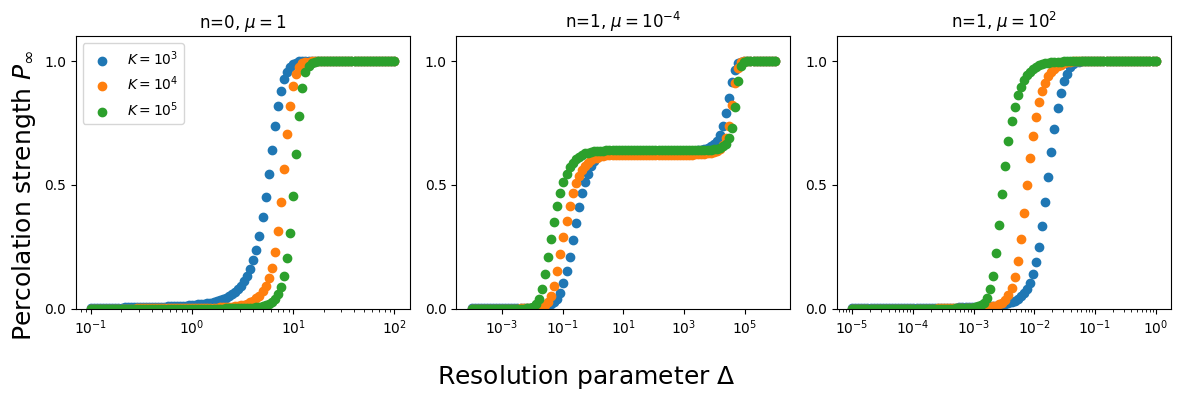
\includegraphics[width=0.95\textwidth]{phase_article_R=1000.png}
    \caption{Percolation phase diagrams for different event number $K$ taking average values of $R=1000$ realizations.}
    \label{f:phase_diagram_article}
\end{figure}

The first plot configuration is a Markovian ($n=0$) Poisson process with rate $\mu$. This is the simplest case, where the inter-event time $x=t_i-t_{i-1}$ follows an exponential 
distribution $P(x_i)=\mu e^{\mu x_i}$. The other two plots are non-Markovian Hawkes processes for $\mu \ll 1$ and $\mu\gg 1$. In one hand, a double transition is observed when 
$\mu = 10^{-4}$, in the other hand, a single transition occurs when $\mu = 10^2$. 

After the phase diagram is 